\section{Evaluation}

\subsection{Detailed evaluation of examples}

Let us consider the following example:
$\alpha_1 = \{x_1 - x_2 \geq -4, -x_2 - x_3 \geq 5, 
  x_2 + x_6 \geq 4, x_2 + x_5 \geq -3\}; 
\beta_1 = \{-x_1 + x_3 \geq -2, -x_4 - x_6 \geq 0, -x_5 + x_4 \geq 0\}$. 

The output obtained by our implementation is
(and ($\leq$ (- (- x6) x1) 0)
($\leq$ (+ (- x6) x3) (- 9))
($\leq$ (- (- x5) x1) 7)
($\leq$ (+ (- x5) x3) (- 2)))).
and produced the following trace
for this problem:

\verbatiminput{../../Software/Cpp/OctagonsInterpolant/tests/traces/example1.txt}

The Z3 SMT solver provides mechanisms to modify the arithmetic engine 
and several plugins to specialize algorithm for specific theories. It contains a
proper specialization to work with UTVPI queries for satisfiability checking. 
However,  the interpolation APIs do not include mechanisms to specialize the 
interpolation algorithm for UTPVI formulas, i.e. Z3 does produce interpolant
in the UTVPI theory.
Thus, the interpolant obtained by Z3 for the above problem is : 
(and ($\leq$ 9 (+ (* (- 1) x3) (* 2 x6) x1)) ($\leq$ (- 5) (+ (* (- 1) x3) (* 2 x5) x1))).
We can notice by the coefficients in the result that the interpolant is not
a UTVPI formula, thus Z3 must have reduced the problem to linear integer arithmetic.

The result obtained by Mathsat is 
(and ($\leq$ (- 5) (+ x1 (+ (* (- 1) x3) (* 2 x5)))) ($\leq$ 9 (+ x1 (+ (* (- 1) x3) (* 2 x6))))) 
which is the same as Z3 modulo the commutativity of the
additions in the expression. Despite this difference, the following query 
to Z3 verifies that the interpolation produced by our implementation implies 
the interpolation produced by the SMT solver above mentioned; at the same time,
the interpolant produced by the SMT solver does not imply our interpolant.

\verbatiminput{../../Software/Cpp/OctagonsInterpolant/verification/example1_strongest_inter_verification.smt2}

For the next example, let us consider $\alpha_2 = \{
  -x_2 - x_1 + 3 \geq 0, 
  x_1 + x_3 + 1 \geq 0, 
  -x_3 - x_4 - 6 \geq 0, 
  x_5 + x_4 + 1 \geq 0 
\}; \beta_2 = \{
  x_2 + x_3 + 3 \geq 0,
  x_6 - x_5 - 1 \geq 0,
  x_4 - x_6 + 4 \geq 0
\}$. 

Our implementation produced the followint output
(and
($\leq$ (+ (- x3) x2) 4)
($\leq$ (+ x4 x3) (- 6))
($\leq$ (- (- x5) x4) 1)).
and obtained the following trace:

\verbatiminput{../../Software/Cpp/OctagonsInterpolant/tests/traces/example2.txt}

The interpolant obtained by Z3 is 
(and ($\leq$ (- 4) (+ x3 (* (- 1) x2))) ($\leq$ (+ x3 x4) (- 6)) ($\geq$ (+ x4 x5) (- 1))); 
and the interpolant produced by Mathsat is ($\leq$ (+ x2 (+ x3 (+ x4 (* (- 1) x5)))) (- 7)).
Using Z3, we were able to verify that: 
\begin{itemize}
  \item the interpolantion obtained by our implementation
    is equivalent to the interpolant obtained by Z3. 
  \item the interpolant obtained by our implementation implies the interpolant
    obtained by Mathsat, but the converse does not hold.
\end{itemize}

\verbatiminput{../../Software/Cpp/OctagonsInterpolant/verification/example2_strongest_inter_verification.smt2}

\subsection{Performance comparison with iZ3 and MathSat}\label{performance_oct}

This section discusses a benchmark of interpolation 
generation for the UTVPI theory. Similarly to the previous chapter,
we compare the performance of our tool with respect to the
iZ3 and Mathsat.

\subsubsection{Benchmark description}

The benchmark contains the following parameters:

\begin{itemize}
  \item $l$ stands for a random number of the max value
    of the bounds
  \item $m$ stands for the number of variables allowed
    in the random signature
  \item $n$ stands for the number of inequalities of the
    form: $a_1 x_{k_1} + a_2 x_{k_2} \leq c$
    or $a_1 x_{k_1} - a_2 x_{k_2} \leq c$
    where $a_1, a_2$ are chosen
    uniformly at random from the set of elements
    $\{-1, 0, 1\}$, $k_1, k_2$ are chosen uniformly
    at random from the the set of elements 
    $\{1, \dots, n\}$, and $c$ is chosen uniformly
    at random from the set $\{-l, \dots, l\}$
\end{itemize}

We constructed a pair of inconsistent formulas $(A-part, B-part)$
using an identical construction to the benchmark proposed in 
the previous chapter, using two $z3: :solver$ in order to maintain
each $A-part$ and $B-part$ consistent but inconsistent with 
each other. 

\subsubsection{Experimental results}

We designed the problem becuase the randomness makes it
difficult to come up with trivial solutions. This problem 
was executed $100$ and $10000$ times using the parameters
$(l = 1000, m = 10, n = 5)$ and 
$(l = 10, m = 10, n = 20)$ respectively.

The following graph reports the time needed
by our implementation, iZ3, and the interpolation 
generation algorithm from Mathsat. 
It is well known that both iZ3 and Mathsat does not
compute uniform interpolants for UTVPI. 
Regardless, the benchmark
was used with the purpose to compare their execution time
on normal interpolants.

\begin{figure}
  \centering
  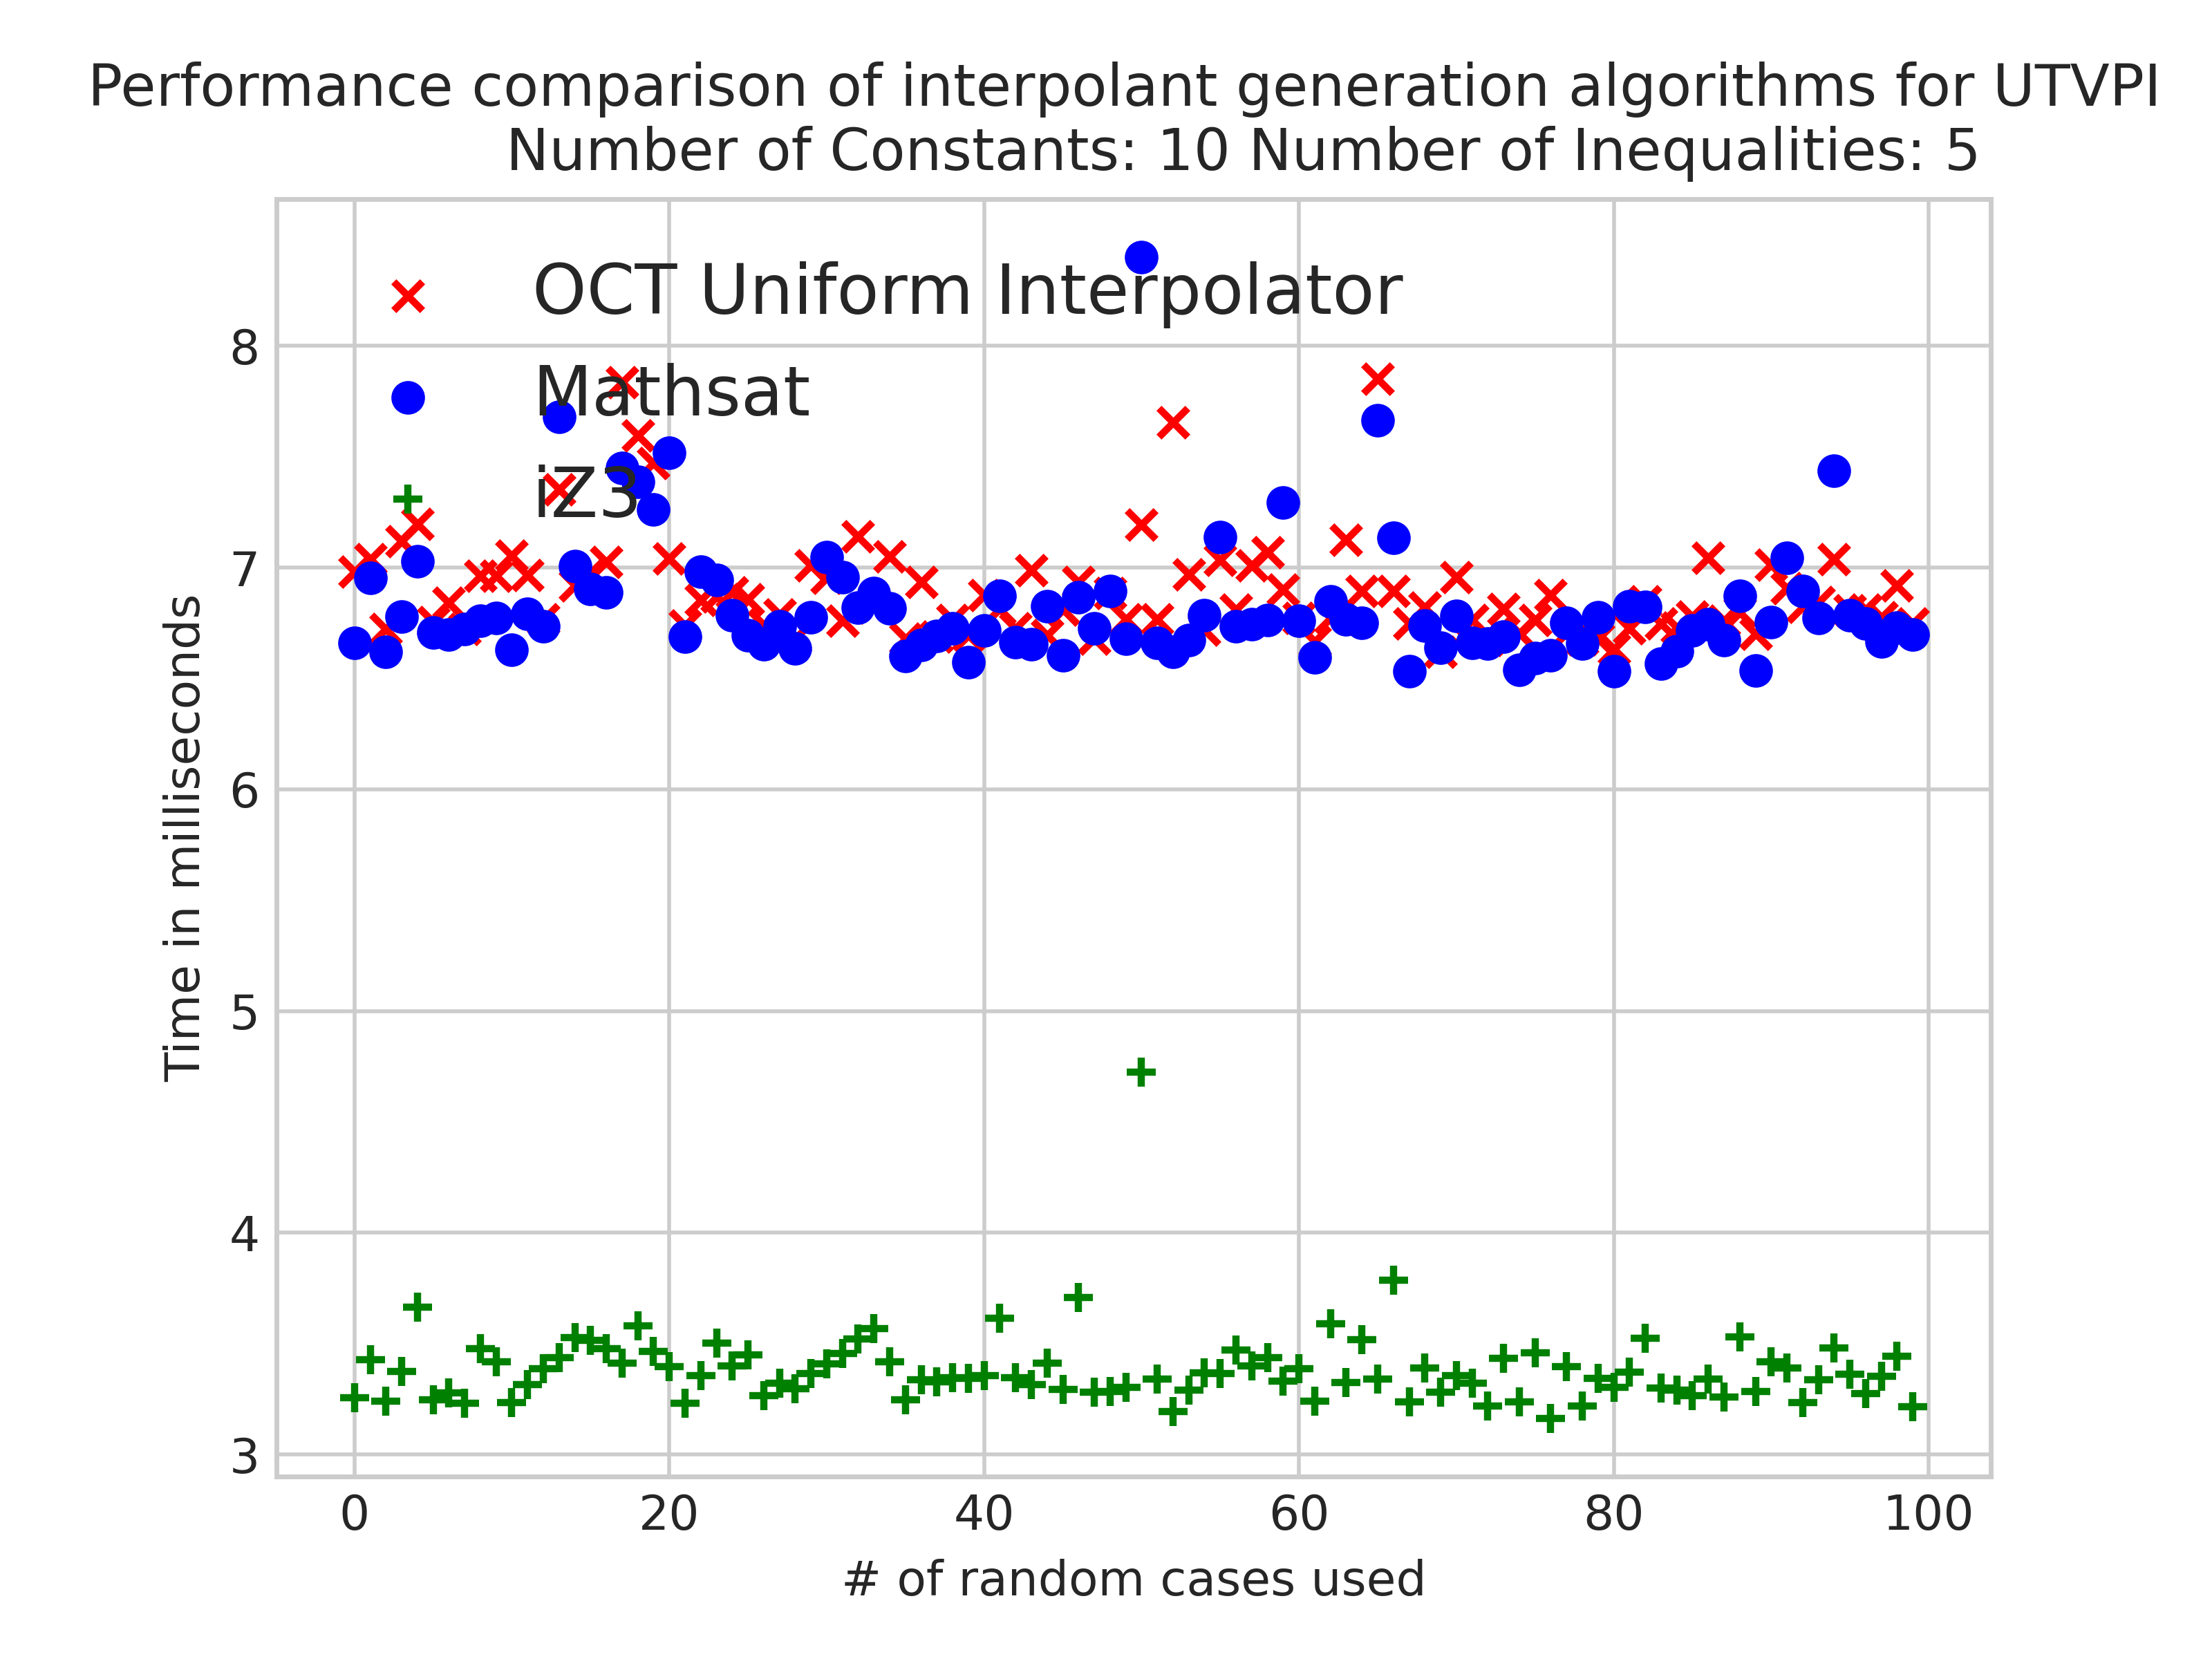
\includegraphics[scale=0.6]{figures/octi_performance_graph_10_5_100}
  \caption{Performance comparison graph of UTVPI interpolant generation
  algorithms for the benchmark (l = 1000, m = 10, n = 5)}
  \label{performance_graph_oct}
\end{figure}

\begin{figure}
  \centering
  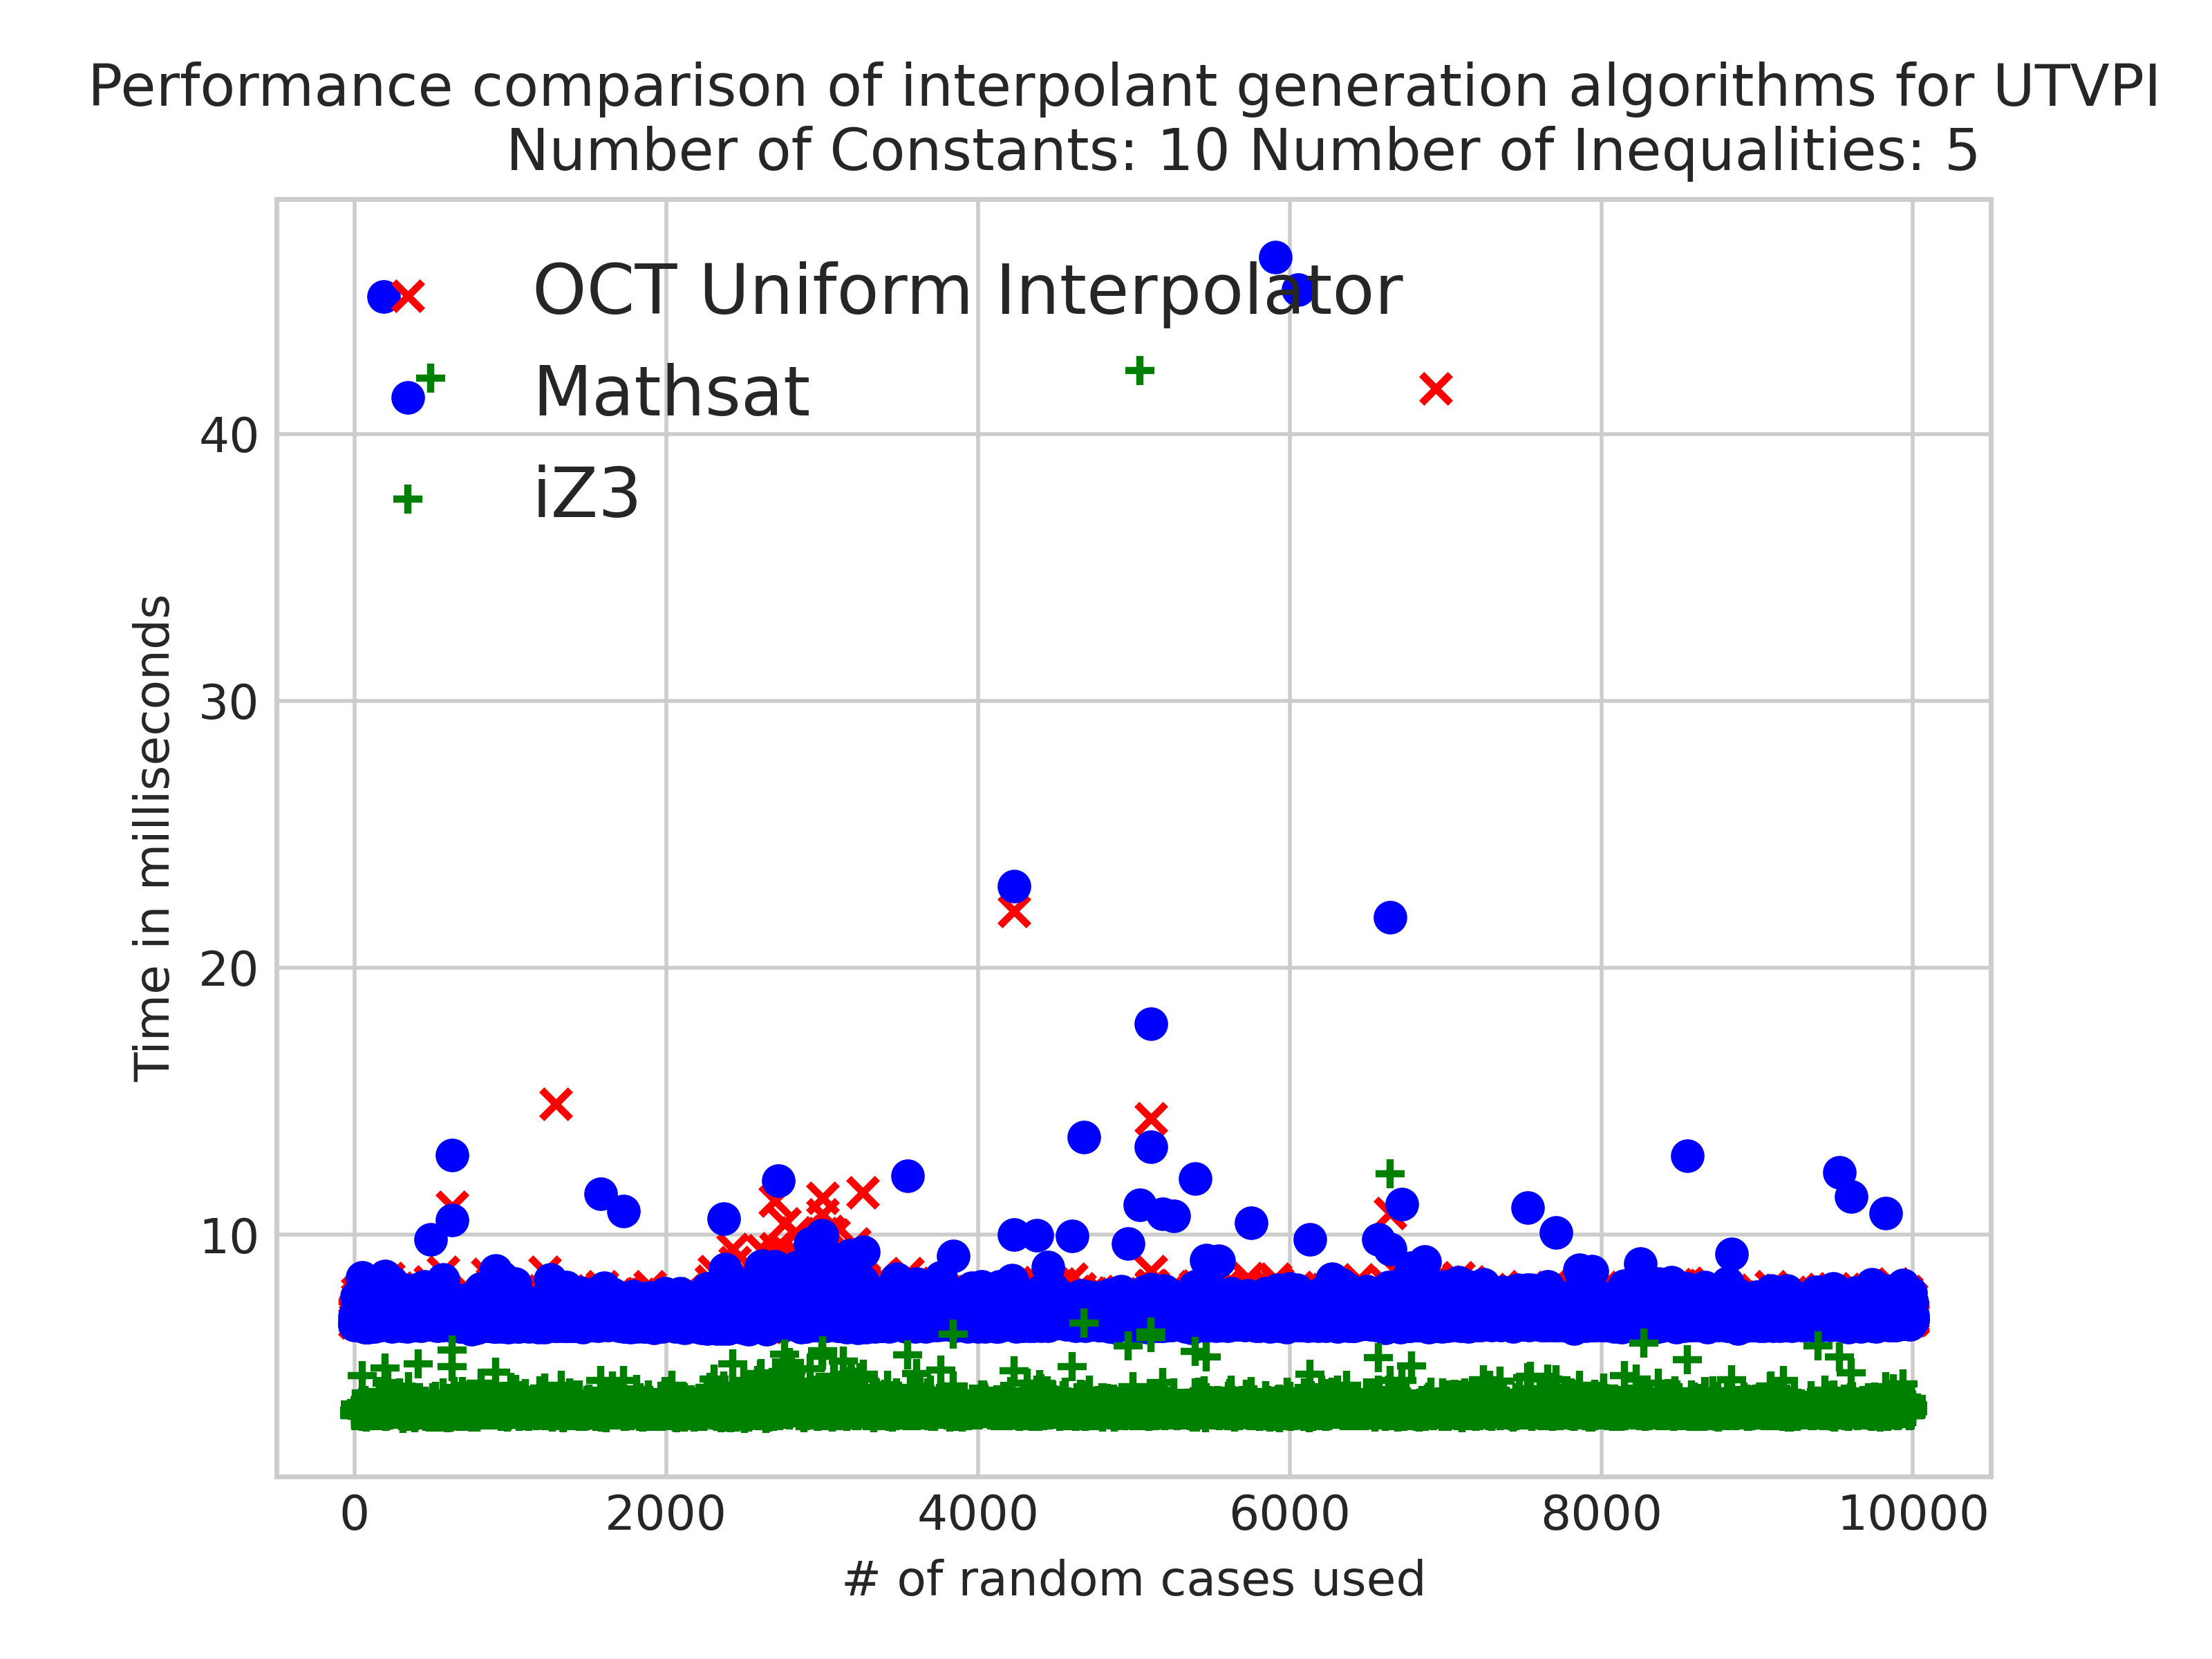
\includegraphics[scale=0.6]{figures/octi_performance_graph_10_5_10000}
  \caption{Performance comparison graph of UTVPI interpolant generation
  algorithms for the benchmark (l = 1000, m = 10, n = 5)} 

  \label{performance_graph_oct_2}
\end{figure}

\begin{figure}
  \centering
  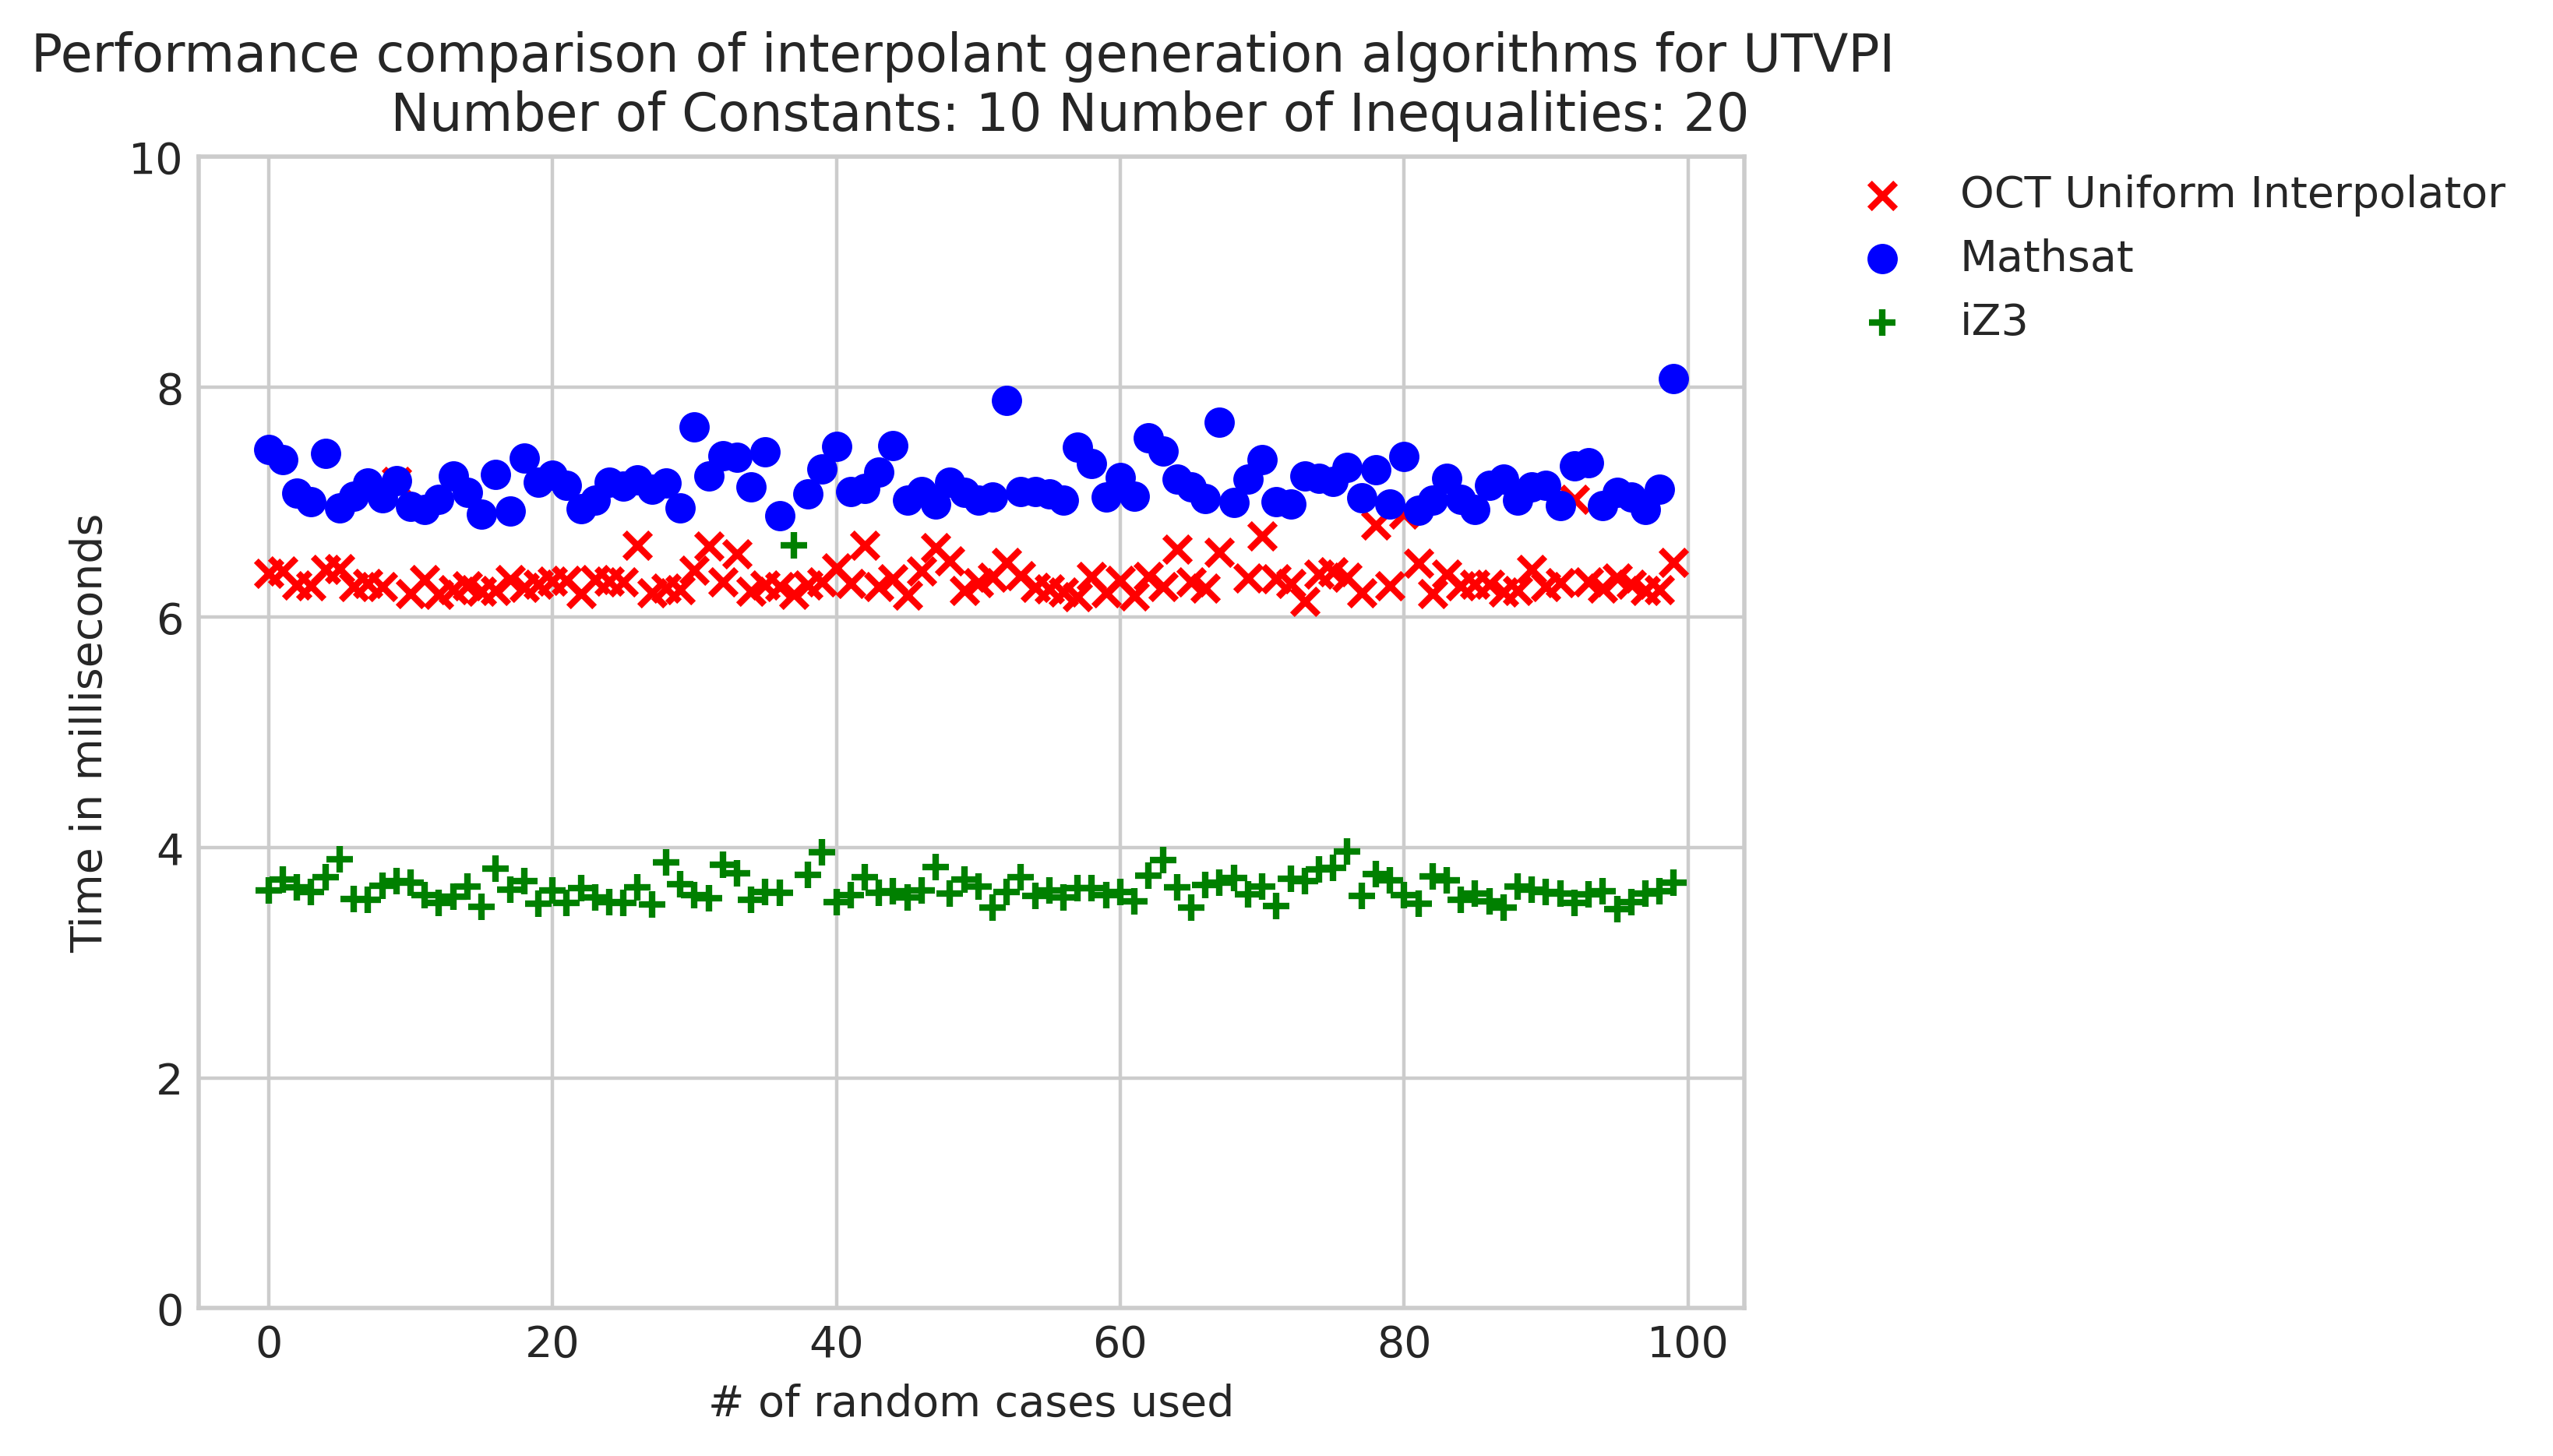
\includegraphics[scale=0.6]{figures/octi_performance_graph_10_20_100.png}
  \caption{Performance comparison graph of UTVPI interpolant generation
  algorithms for the benchmark (l = 1000, m = 10, n = 20)} 

  \label{performance_graph_oct_3}
\end{figure}

\begin{figure}
  \centering
  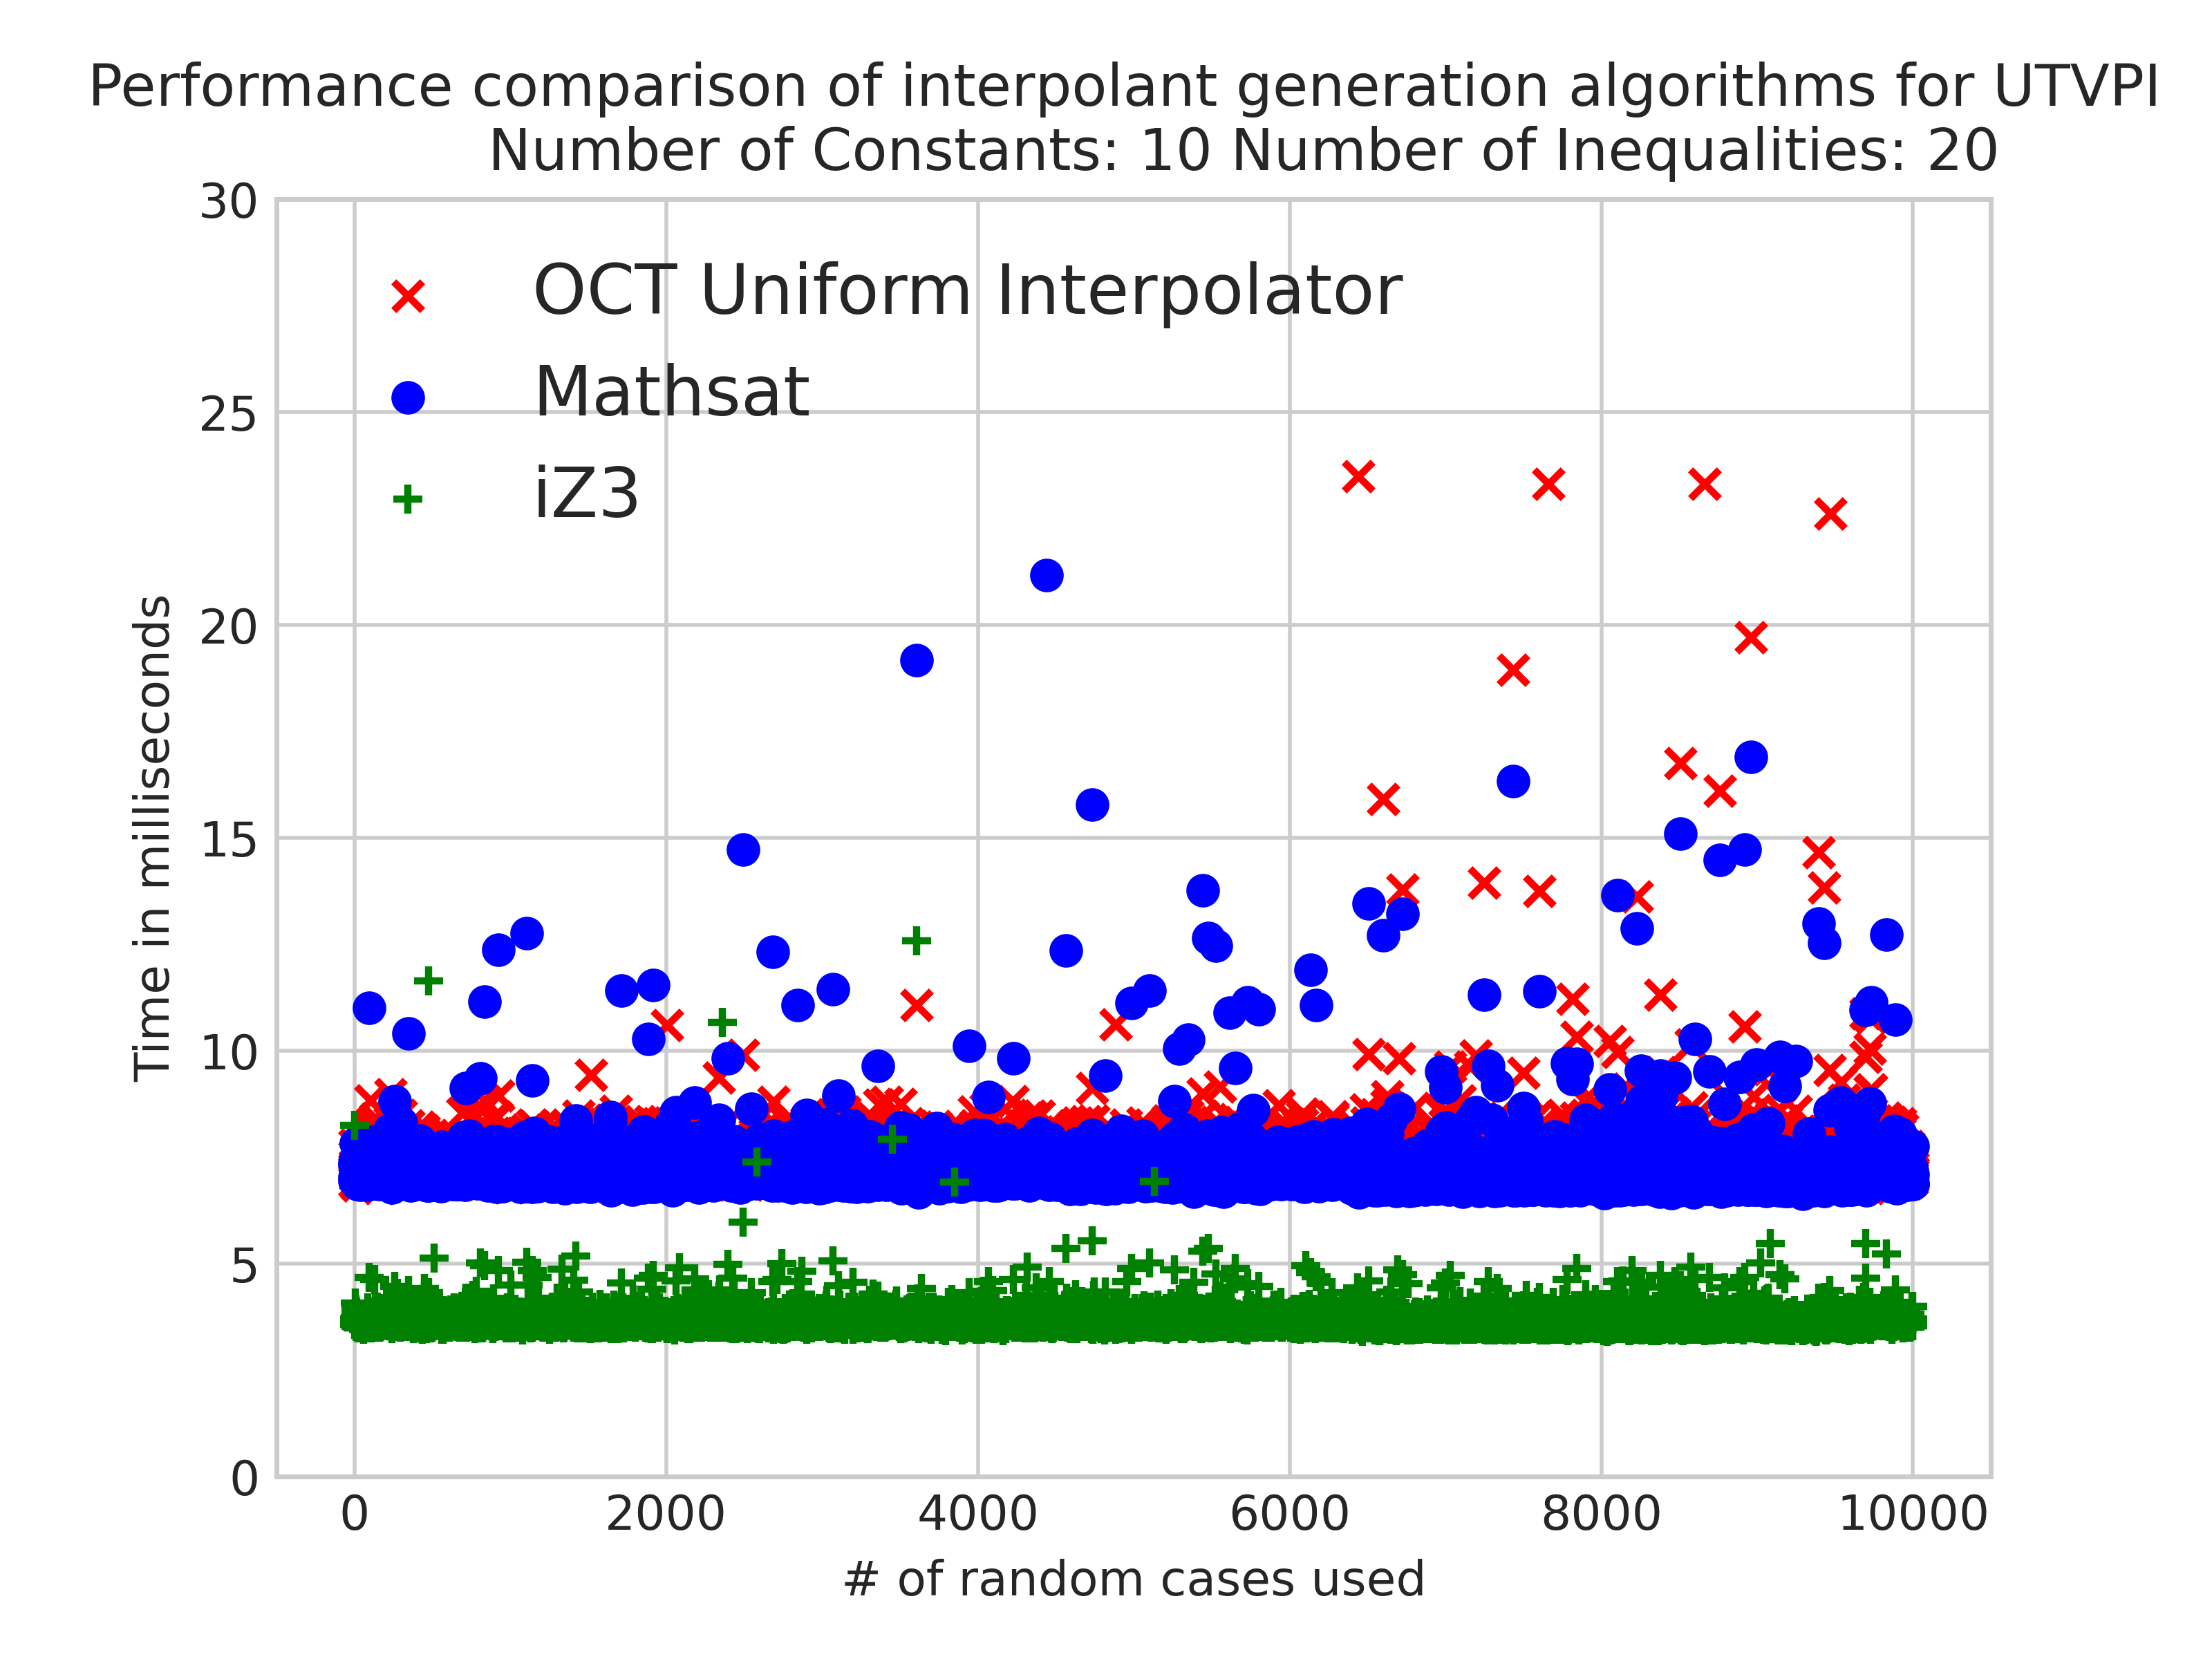
\includegraphics[scale=0.6]{figures/octi_performance_graph_10_20_10000.png}
  \caption{Performance comparison graph of UTVPI interpolant generation
  algorithms for the benchmark (l = 1000, m = 10, n = 20)} 

  \label{performance_graph_oct_4}
\end{figure}

%%% Local Variables:
%%% mode: latex
%%% TeX-master: "main"
%%% End:


%%% Local Variables:
%%% mode: latex
%%% TeX-master: "main"
%%% End:
